\documentclass{article}
\usepackage[left=2cm,right=2cm,top=2cm,bottom=2cm]{geometry}
\usepackage[utf8]{inputenc}
\usepackage[german]{babel}
\usepackage{amsmath}
\usepackage{dsfont}
\usepackage[export]{adjustbox}
\usepackage{amsthm}
\usepackage{color}
\usepackage{amsfonts}
\usepackage{amssymb}
\usepackage{wasysym}
\usepackage{makeidx}
\usepackage{graphicx}
\usepackage[colorlinks=true,urlcolor=blue,linkcolor=blue]{hyperref}
\usepackage{ziffer}
\usepackage{minted}
\usepackage{xcolor}
\usepackage{framed}
\usepackage{mdframed}
\usepackage{subfiles}
\usemintedstyle{emacs}

\definecolor{purp}{HTML}{9A72AC}
\definecolor{re}{HTML}{FC6255}
\definecolor{gre}{HTML}{83C167}
\definecolor{blu}{HTML}{58C4DD}
\definecolor{shadecolor}{rgb}{0.85,0.85,0.85}
\definecolor{bg}{rgb}{0.95,0.95,0.95}
\setlength{\parindent}{0em} 

\BeforeBeginEnvironment{minted}{\begin{mdframed}[linewidth =2 ,backgroundcolor=bg , linecolor=black, linewidth=0.5]}
\AfterEndEnvironment{minted}{\end{mdframed}}

\newtheorem{defi}{Definition}
\BeforeBeginEnvironment{defi}{\begin{mdframed}[linewidth =2 ,backgroundcolor=bg , linecolor=black, linewidth=0.5]}
\AfterEndEnvironment{defi}{\end{mdframed}}

\newcommand{\bsp}{\textbf{Beispiel}:}
%\newcommand{\task}{\textbf{Aufgabe}:}

\newcommand{\bol}[1]{\textbf{#1}}
\newcommand{\q}[1]{\glqq #1\grqq}
\newcommand{\DODO}[1]{\textbf{\textcolor{red}{DODO:}} #1 \\ \begin{center}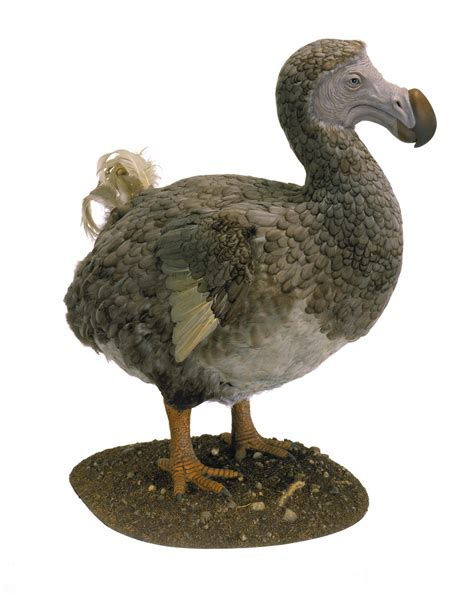
\includegraphics[scale=0.2]{../../media/dodo.jpg} \end{center}}

\newenvironment{task}[1]{
    \begin{shaded*}
    \textbf{Aufgabe #1}:
}{
    \end{shaded*}
}

\begin{document}
\subsection{Entwurfsmuster}

\begin{center}
    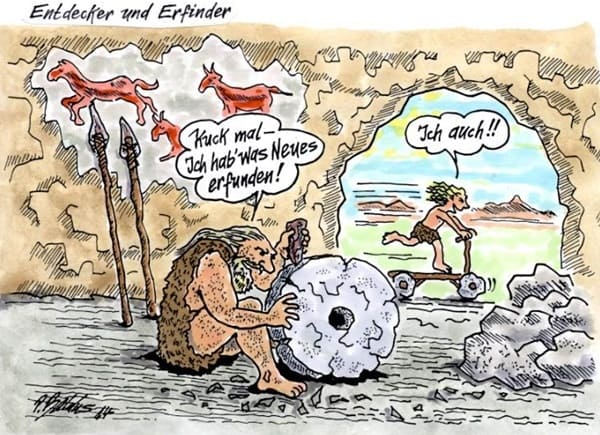
\includegraphics[scale=0.5]{../../media/cartoon_rad.jpg} \\
    \textit{Quelle:} \href{https://www.lehrer-online.de/artikel/fa/cartoon-der-woche-entdecker-und-erfinder/#}{lehrer-online}
\end{center}

Wäre dies ein Skript zu einem anderen Fach, so wäre die erste Aufgabe die Analyse des obigen Comics. Glücklicher-weise ist das in Informatik nicht notwendig - die Kernaussage ist klar. Zwar ist es durchaus nützlich für das Verständnis, Dinge selbst zu programmieren, aber Zeit ist eine begrenzte Ressource. Deswegen ist es unerlässlich, dass auf die Arbeit von von anderen Personen zurückgegriffen wird. Möchte man fremden Code nicht direkt kopieren - oder kann das nicht, weil er doch nicht zu 100 Prozent auf den eigenen Fall zutrifft - so kann man sich zumindest an der Art und Weise der Problemlösung orientieren. \\
Da es Problemklassen gibt, die häufig ein ähnliches Vorgehen erfordern, wurden bereits Lösungsschablonen entwickelt, die im Allgemeinen \textbf{Entwurfsmuster} heißen. Das bedeutet, dass ein grobes Klassendiagramm der Struktur bereits vorhanden ist, eine konkrete Ausgestaltung ist aber dem Programmiery überlassen. \\
Wir haben bereits mit dem \textbf{Kompositum} ein Entwurfsmuster kennengelernt, auch dort haben wir nicht direkt \q{\textbf{Das Kompositum}} implementiert, sondern die grundlegende Idee, die dahinter steckt, verwendet. \\
Es gibt noch unzählige weitere Entwurfsmuster, hier eine kleine Auswahl, jeweils mit kurzer Erläuterung:

\begin{itemize}
    \item \textbf{Singleton}: stellt sicher, dass von der betrachteten Klasse nur ein einziges Objekt erzeugt werden kann und bietet eine globale Zugriffsmöglichkeit auf dieses Objekt. Z.B. braucht ein Login-System nur eine Instanz (dieses soll alle Logins verwalten!).
    \item \textbf{Factory}: Abstrahiert die Erstellung von Objekten, indem sie eine gemeinsame Schnittstelle für die Erstellung von Objekten definiert und die spezifische Omplementierung der Objekterstellung in weitere Unterklassen auslagert. Dieses Muster kann z.B. bei der Erstellung von Spielfiguren o.Ä. nützlich sein.
    \item \textbf{Observer}: stellt eine Möglichkeit bereit, um auf Änderungen eines Objekts zu reagieren, indem andere Objekte (die Observer) benachrichtigt werden. Ein klassischer Anwendungsfall wäre ein Benachrichtigungsticker (siehe auch Benachrichtigungen am Handy!).
    \item \textbf{Decorator}: ermöglicht die dynamische Erweiterung von Objekten durch Hinzufügen von zusätzlichen Funktionen oder Eigenschaften (die Dekorationen). Ein Bild kann z.B. mit Filtern \q{dekoriert} werden.
    \item \textbf{Adapter}: ermöglicht die Integration von inkompatiblen Klassen durch die Entwicklung einer gemeinsamen Schnittstelle (sehr allgemeines Konzept!).
    \item \textbf{Iterator}: es wird eine Möglichkeit bereitgestellt, sequentiell auf Elemente in einer Zusammenstellung zuzugreifen, z.B. in einer Liste. 
\end{itemize}

Das Muster, das für unser Projekt zentral sein soll, ist noch etwas allgemeiner als die Meisten der oben bereits erwähnten - \textbf{Model View Controller}. Es kann sich nicht nur auf einzelne Klassen beziehen (auch wenn das durchaus möglich ist), sondern beschreibt die grundlegende Implementierungsidee einer ganzen \textbf{Softwarearchitektur}. \\
Bevor wir uns Beispielen zuwenden ein kurzer Überblick über die drei Komponenten:
\begin{enumerate}
    \item \textbf{Modell (Model)}: Das Modell beschreibt die konkreten Daten, die mit dieser Anwendung verknüpft sind. Die Daten können dabei in vielerlei Form vorliegen, von definierten Attributen in einfachen Klassen über Datenformate wie \textbf{\href{https://de.wikipedia.org/wiki/JavaScript_Object_Notation}{JSON}} bis hin zu ganzen Datenbanken. Hier kann gegebenenfalls auch noch Logik implementiert sein, wenn die Daten, z.B. bei Speicherung, noch verarbeitet werden müssen.
    \item \textbf{Ansicht (View)}: Die Ansicht ist dazu da, die Daten des Modells in einer Form darzustellen, sodass der Anwender mit ihnen interagieren kann. Letztendlich läuft es im modernen Kontext in der Regel auf ein \textbf{Graphical User Interface (GUI)} hinaus. GUIs verwenden häufig das Entwurfsmuster Kompositum, da sie aus Komponenten mit ähnlichen Grundfunktionen (z.B. Menüeintrag, klickbares Objekt, Datendarstellung etc.) zusammengesetzt werden. 
    \item \textbf{Steuerung (Controller)}: Die Steuerung verwaltet die anderen beiden Komponenten. In der Regel wird das Entwurfsmuster \q{Observer} verwendet, um auf Interaktion des Anwenders mit der Ansicht zu \q{\textbf{lauschen}}. Anschließend veranlasst die Steuerung alle notwendigen Änderungen, so werden beispielsweise neue Menüeinträge angezeigt, oder neue Daten werden von einem Eingabefeld in der 
\end{enumerate}

In einem sehr vereinfachten Schema mit jeweils einer Klasse dargestellt:
\begin{center}
    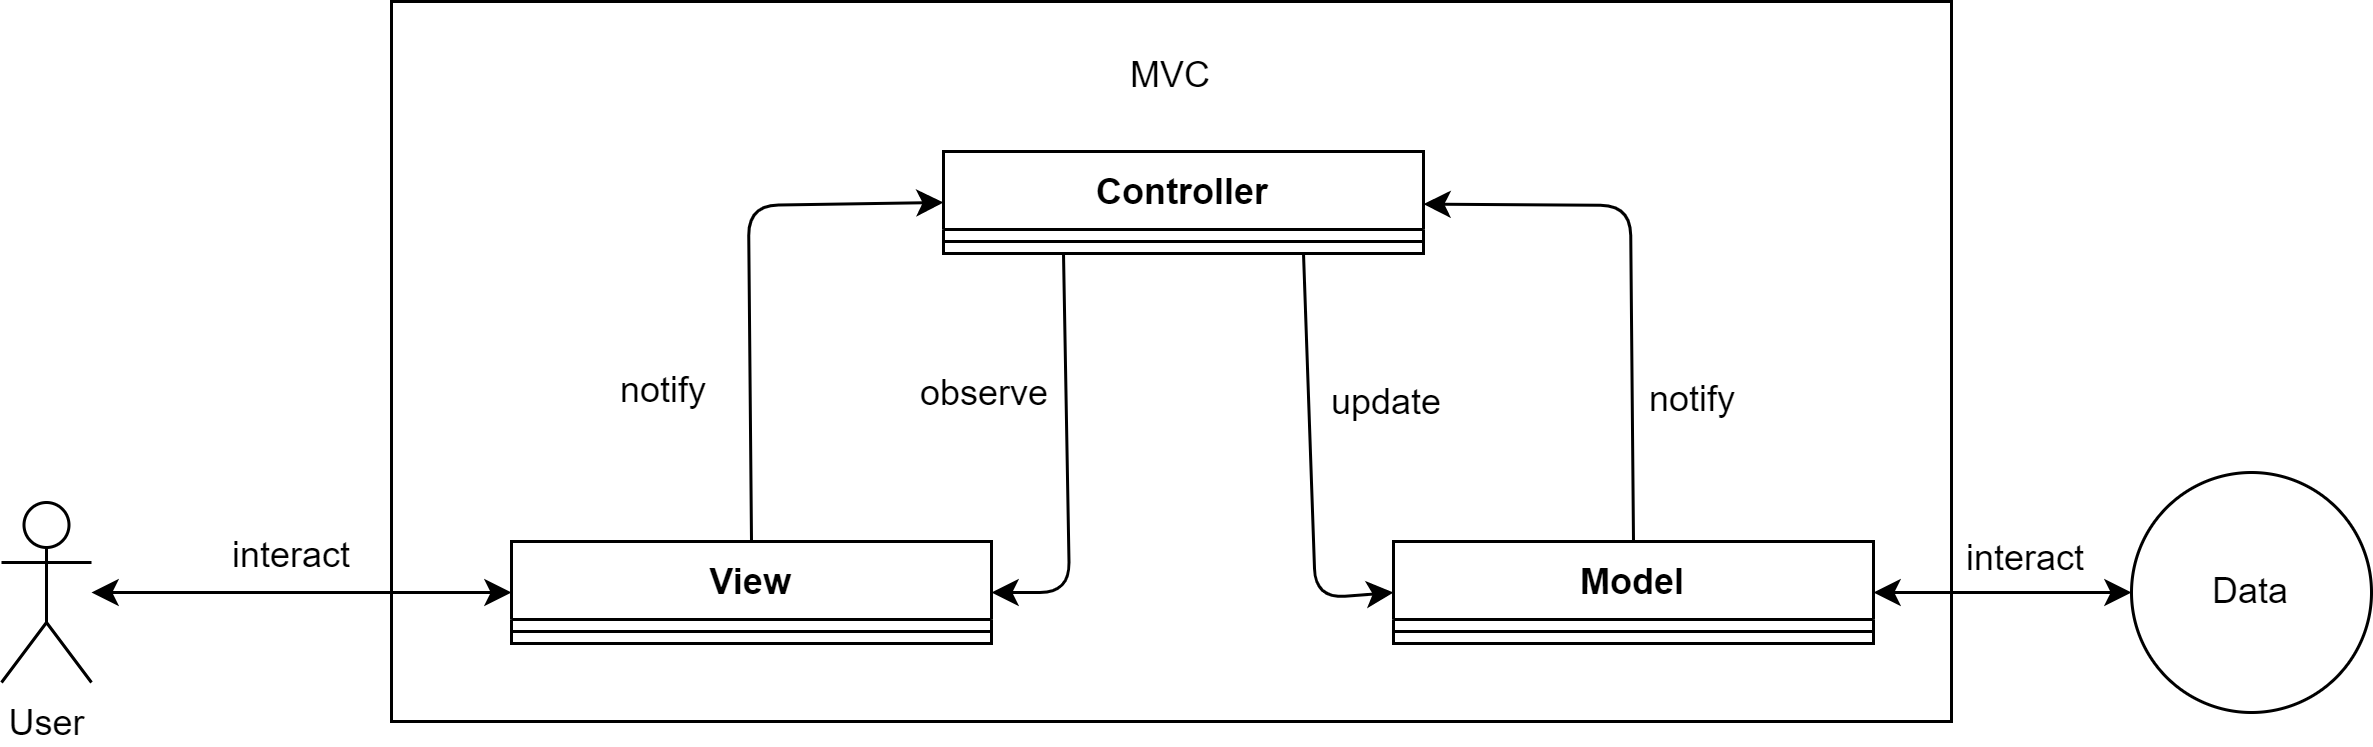
\includegraphics[scale=0.2]{../../media/mvc.png}
\end{center}
Ein mögliches Grundgerüst der Implementierung dieses Diagramms sieht so aus: 

\begin{minted}{java}
//Unser Model entspricht hier einfach nur einer Datenklasse, die Zugriff und
//Änderungen regelt.
public class Model {
    private String data;

    public String getData() {
        return data;
    }

    public void setData(String data) {
        this.data = data;
    }
}

public class Controller {
    //Der Controller hat Referenzen auf ein Model und einen View
    private Model model;
    private View view;

    //Der Controller könnte Model und View im Konstruktur auch direkt 
    //erzeugen - man könnte hier auch das Singleton-Pattern verwenden,
    //wenn man sichergehen möchte, dass in einer Instanz des Programms
    //nur ein Controller existieren kann!
    public Controller(Model model, View view) {
        this.model = model;
        this.view = view;
    }

    //Um Daten zu modifizieren (z.B. durch eine Eingabe im View getriggert)
    //mus der Controller auch auf die Methoden des Models zugreifen:
    public void setData(String data) {
        model.setData(data);
    }

    public String getData() {
        return model.getData();
    }

    //Der View wird mit dieser Methode aktualisiert, d.h. hier:
    //Die aktuellen Daten werden auf der Konsole ausgegeben.
    public void updateView() {
        view.printData(model.getData());
    }
}

//Der View ist hier am einfachsten:
//Er gibt einfach nur Daten auf der Konsole aus.
public class View {
    public void printData(String data) {
        System.out.println("Data: " + data);
    }
}
\end{minted}

Diese Implementierung ist noch recht abstrakt, geben wir den Klassen ein klein wenig mehr Leben:
\begin{minted}{java}
//Das Model hat sich nicht wesentlich verändert, es soll jetzt aber 
//einen Spielstand modellieren statt einfach nur eines Textes
public class Model {
    private int score;

    public int getScore() {
        return score;
    }

    public void increaseScore() {
        score += 10;
    }
}

import java.util.Random;

public class Controller {
    private Model model;
    private View view;
    //Um Zufallszahlen zu erzeugen
    private Random random;

    public Controller(Model model, View view) {
        this.model = model;
        this.view = view;
        random = new Random();
    }

    public void performAction() {
        //In diesem kleinen Beispiel wird eine Zufallszahl erzeugt, ist
        //diese gerade, so haben wir "gewonnen" und der Score wird erzeugt
        int randomValue = random.nextInt(10) + 1;
        if (randomValue % 2 == 0) {
            model.increaseScore();
            //außerdem wird angezeigt, dass wir Erfolg hatten!
            view.printSuccessMessage();
        } else {
            //andernfalls wird die Versagens-Meldung angezeigt - Schade :)
            view.printFailureMessage();
        }
        //In jedem Fall wird der derzeitige Spielstand ausgegeben.
        view.printScore(model.getScore());
    }
}

//Der View interagiert weiterhin nur mit der Konsole: 
public class View {
    public void printSuccessMessage() {
        System.out.println("Great job! You earned 10 points.");
    }

    public void printFailureMessage() {
        System.out.println("Sorry, try again.");
    }

    public void printScore(int score) {
        System.out.println("Your current score is: " + score);
    }
}


\end{minted}

Ausgehend von diesen sehr grundlegenden Beispielen können jetzt die einzelnen Klassen sukzessive ausgebaut werden - es muss auch nicht zwingend bei diesen drei Klassen bleiben! Z.B. könnten die Daten in mehreren Klassen organisiert sein. Wollen wir beispielsweise verschiedene Karten modellieren, könnte eine Oberklasse Karte verwendet werden und für die einzelnen speziellen Kartenarten jeweils eine Unterkarte, also z.B. wie bei Uno:
\begin{enumerate}
    \item Zieh Vier Farbwahl
    \item Aussetzen
    \item Richtungswechsel
    \item Zieh 2
    \item Zahlenkarte
\end{enumerate}
Alle erben von Karte, da sie z.B. alle ausgepielt werden können, die Eigenschaften unterscheiden sich aber und sie können spezielle Effekte haben. \\
\textbf{Anmerkung:} Weitere Hinweise zur weiteren Ausdifferenzierung bzw. Ausgestaltung der einzelnen Komponenten finden sich im nächsten Kapitel.

\end{document}